\section{Experimenting and Improving the Agent}
\subsection{Reward-Goal Relationship}\label{sec:reward-goal}
Out goal is to maximize the total distance traveled by the agent. The total discounted return (that the agent tries to maximize) is a proxy for the goal.

\begin{equation}\label{eqn:reward_vanilla}
r(state_t, a_t, state_{t+1}) = \begin{cases}
-5 & \texttt{if control car collides } \\
0.03*s_{t+1} & \texttt{otherwise}
 \end{cases} 
\end{equation}
\begin{align*}
\texttt{Distance} &= \Delta t (s_1 + s_2 + s_3 \dots)\\
\texttt{Discounted Return} &= 0.03 (s_1 + \gamma s_2 + \gamma^ 2 s_3 \dots)
\end{align*}

\begin{enumerate}
    \item While training, we see that sometimes the total discounted return earned increases while total distance traveled decreases. This might happen because the car prioritizes higher speeds earlier and that may lead to a crash. 

    \item As we increases $\gamma \to 1$, the total discounted return is more aligned with the total distance but training becomes unstable, often also reducing performance.
\end{enumerate}

\begin{figure}[H]
    \centering
    \begin{minipage}{0.49\linewidth}
        \centering
        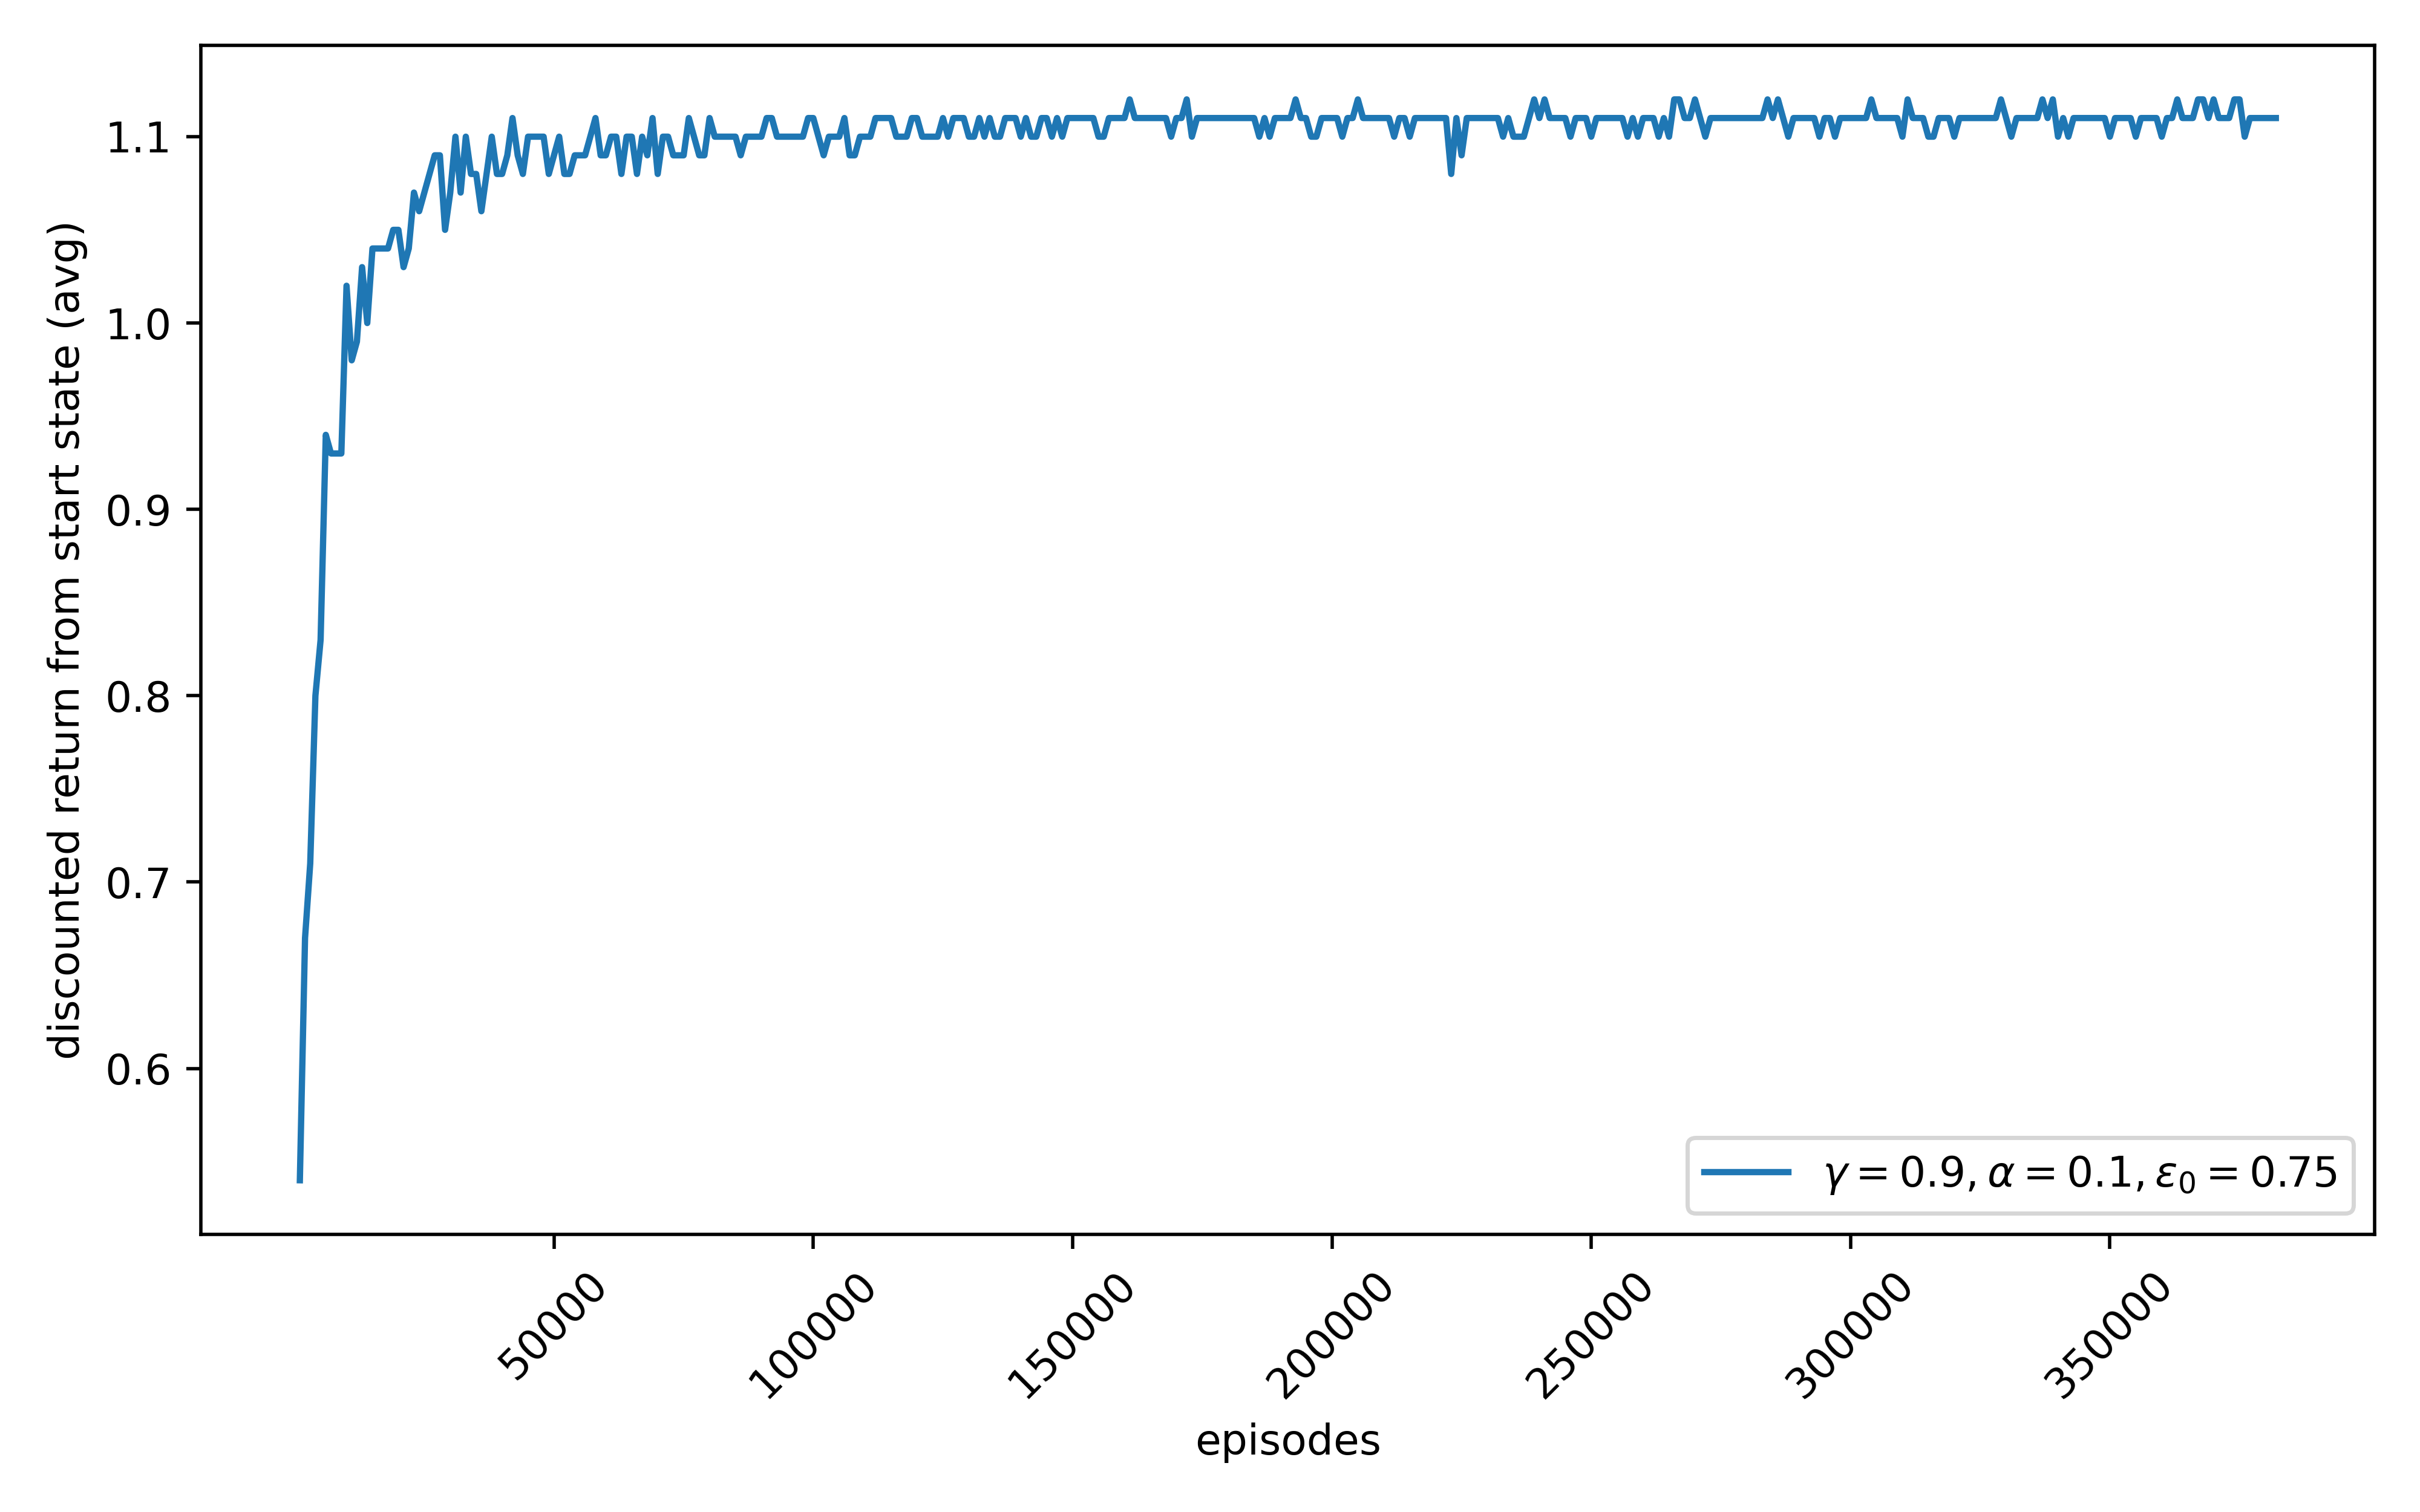
\includegraphics[width=\linewidth]{plots/part3-tabular-bad-rewards.png}
        \caption{Discounted Return}
    \end{minipage}
    \hfill
    \begin{minipage}{0.49\linewidth}
        \centering
        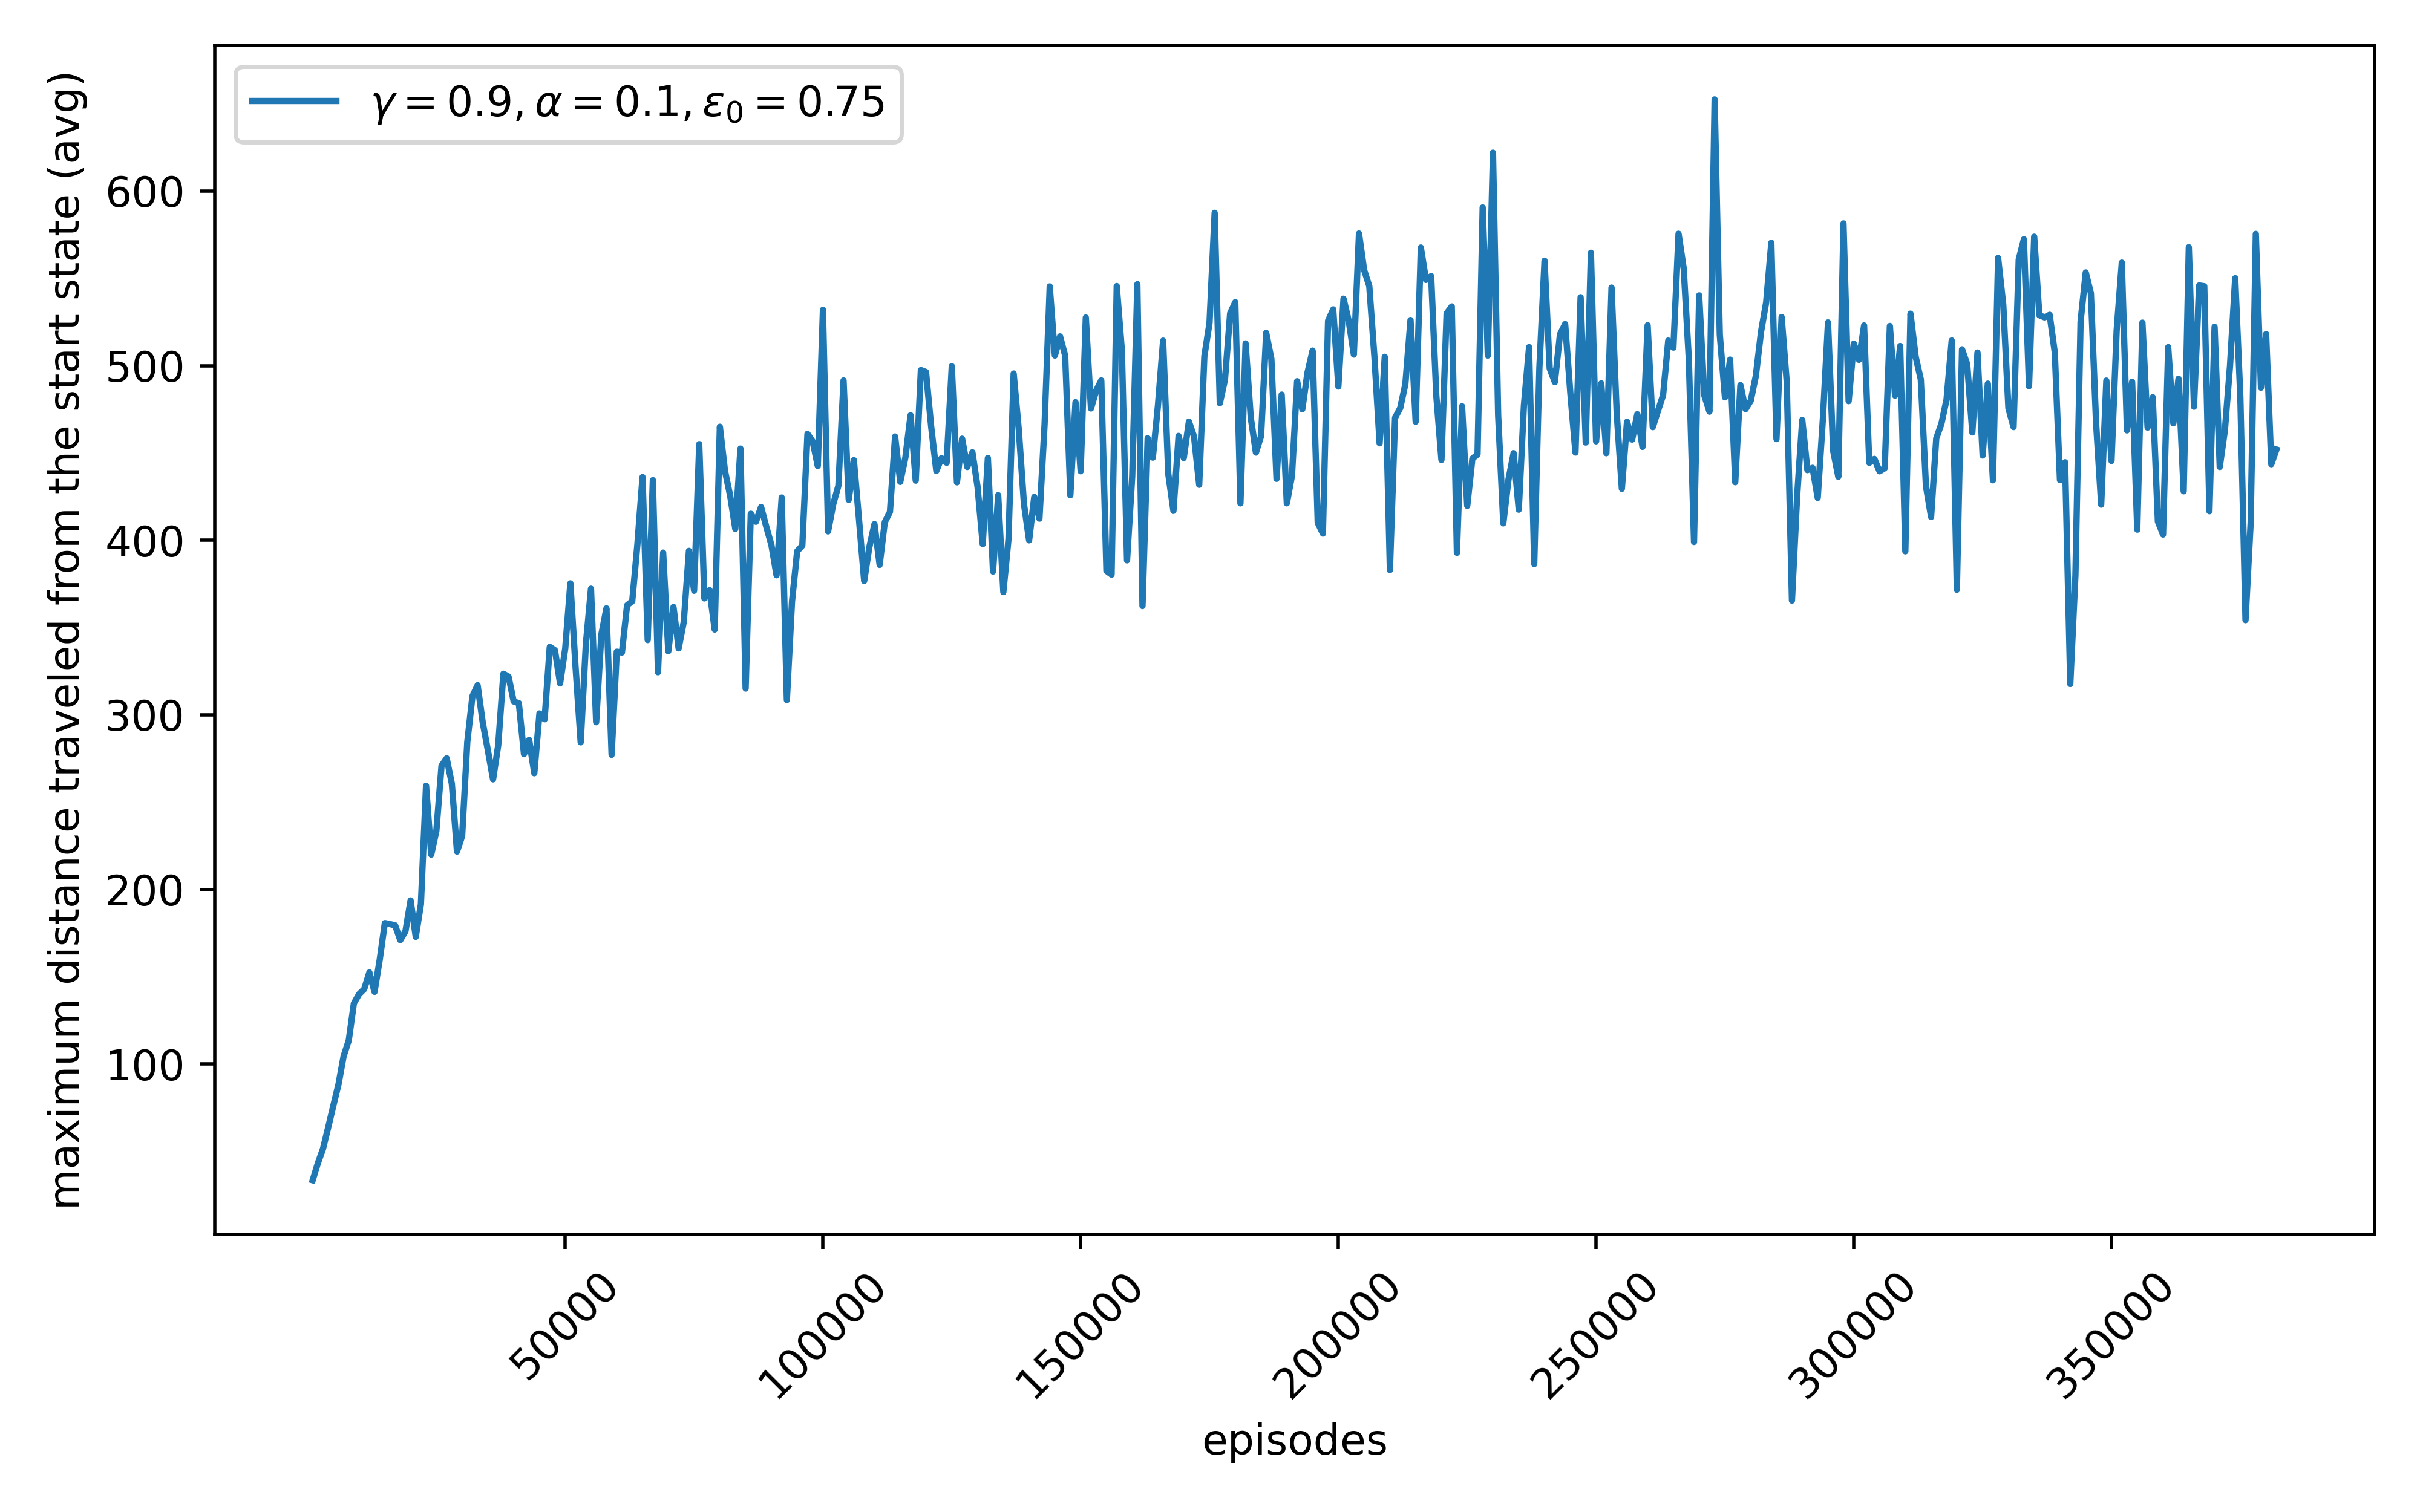
\includegraphics[width=\linewidth]{plots/part3-tabular-bad-distances.png}
        \caption{Distance Traveled}
    \end{minipage}
    \caption{\texttt{Tabular} $\gamma = 0.9, \alpha = 0.1, \epsilon = 0.75$. Further training after $100,000$ iterations does not improve performance.}
    \label{fig:part3-tabular}
\end{figure}

\subsection{Double DQN}
Here, a separate network is used for computing \texttt{target}. This network is updated "slowly". This approach aims to stabilize training. In vanilla DQN, the \texttt{prediction} and \texttt{target} networks both keep moving. 
\begin{align*}
    \texttt{target} &\gets r + \gamma \max_{a'} Q_{target}(s_{t + 1}, a')\\
    \texttt{prediction} &\gets Q_{policy}(s_t, a_t)
\end{align*}
$Q_{policy}$ is trained using gradients. $Q_{target}$ is updated as
\begin{align*}
    \theta_{target} \gets (1 - \tau)  \theta_{target} + \tau \theta_{policy}
\end{align*}
\subsection{Experiments: Optimizers}
\begin{enumerate}
    \item We experimented with \texttt{Adam} and \texttt{AdamW} optimizers with various variations of \texttt{amsgrad}, \texttt{weight\_decay} and $\gamma$ intending that more stable training would allow increasing $\gamma$. The NN architecture used was same as in \nameref{sec:arch}.
    \item We also trained with batch size $512$ but it didn't help. We then moved to a deeper network for the Q-function, described in \nameref{sec:ddqn} leading to the \texttt{DDQN-Vanilla} model.

    \item While training \texttt{DDQN-Vanilla} and \texttt{DDQN-Time-Embed} we also clip gradients to $100$.


\end{enumerate}
\subsection{Designing Reward}\label{sec:reward_design}
\begin{enumerate}
    \item Results in \autoref{tab:part1-d-linear} suggest that linearly decreasing $\epsilon$ works much better than other strategies. In the \texttt{DDQN} case we saw however that the distance traveled down starts going down later. We set a minimum on the $\epsilon$.

    \item To penalize earlier crashes more, we set the reward for crash to
    \begin{equation*}
       \texttt{reward}_{\texttt{crash}} =  -5\left(1 - \frac{\texttt{num\_steps}}{\texttt{episode\_max\_length}}
       \right)
    \end{equation*}
    \item To favor longer runs we add an increasing living reward
        \begin{equation*}
       \texttt{reward}_{\texttt{living}} =  0.15 \frac{\texttt{num\_steps}}{\texttt{episode\_max\_length}}
    \end{equation*}
    \item For the above reward to work, we also add the current timestep as $\left(\frac{\texttt{num\_steps}}{\texttt{episode\_max\_length}}\right)$ to the state. 
\end{enumerate}


\begin{figure}[H]
    \centering
    % First Row - Plots
    \begin{minipage}{0.32\linewidth}
        \centering
        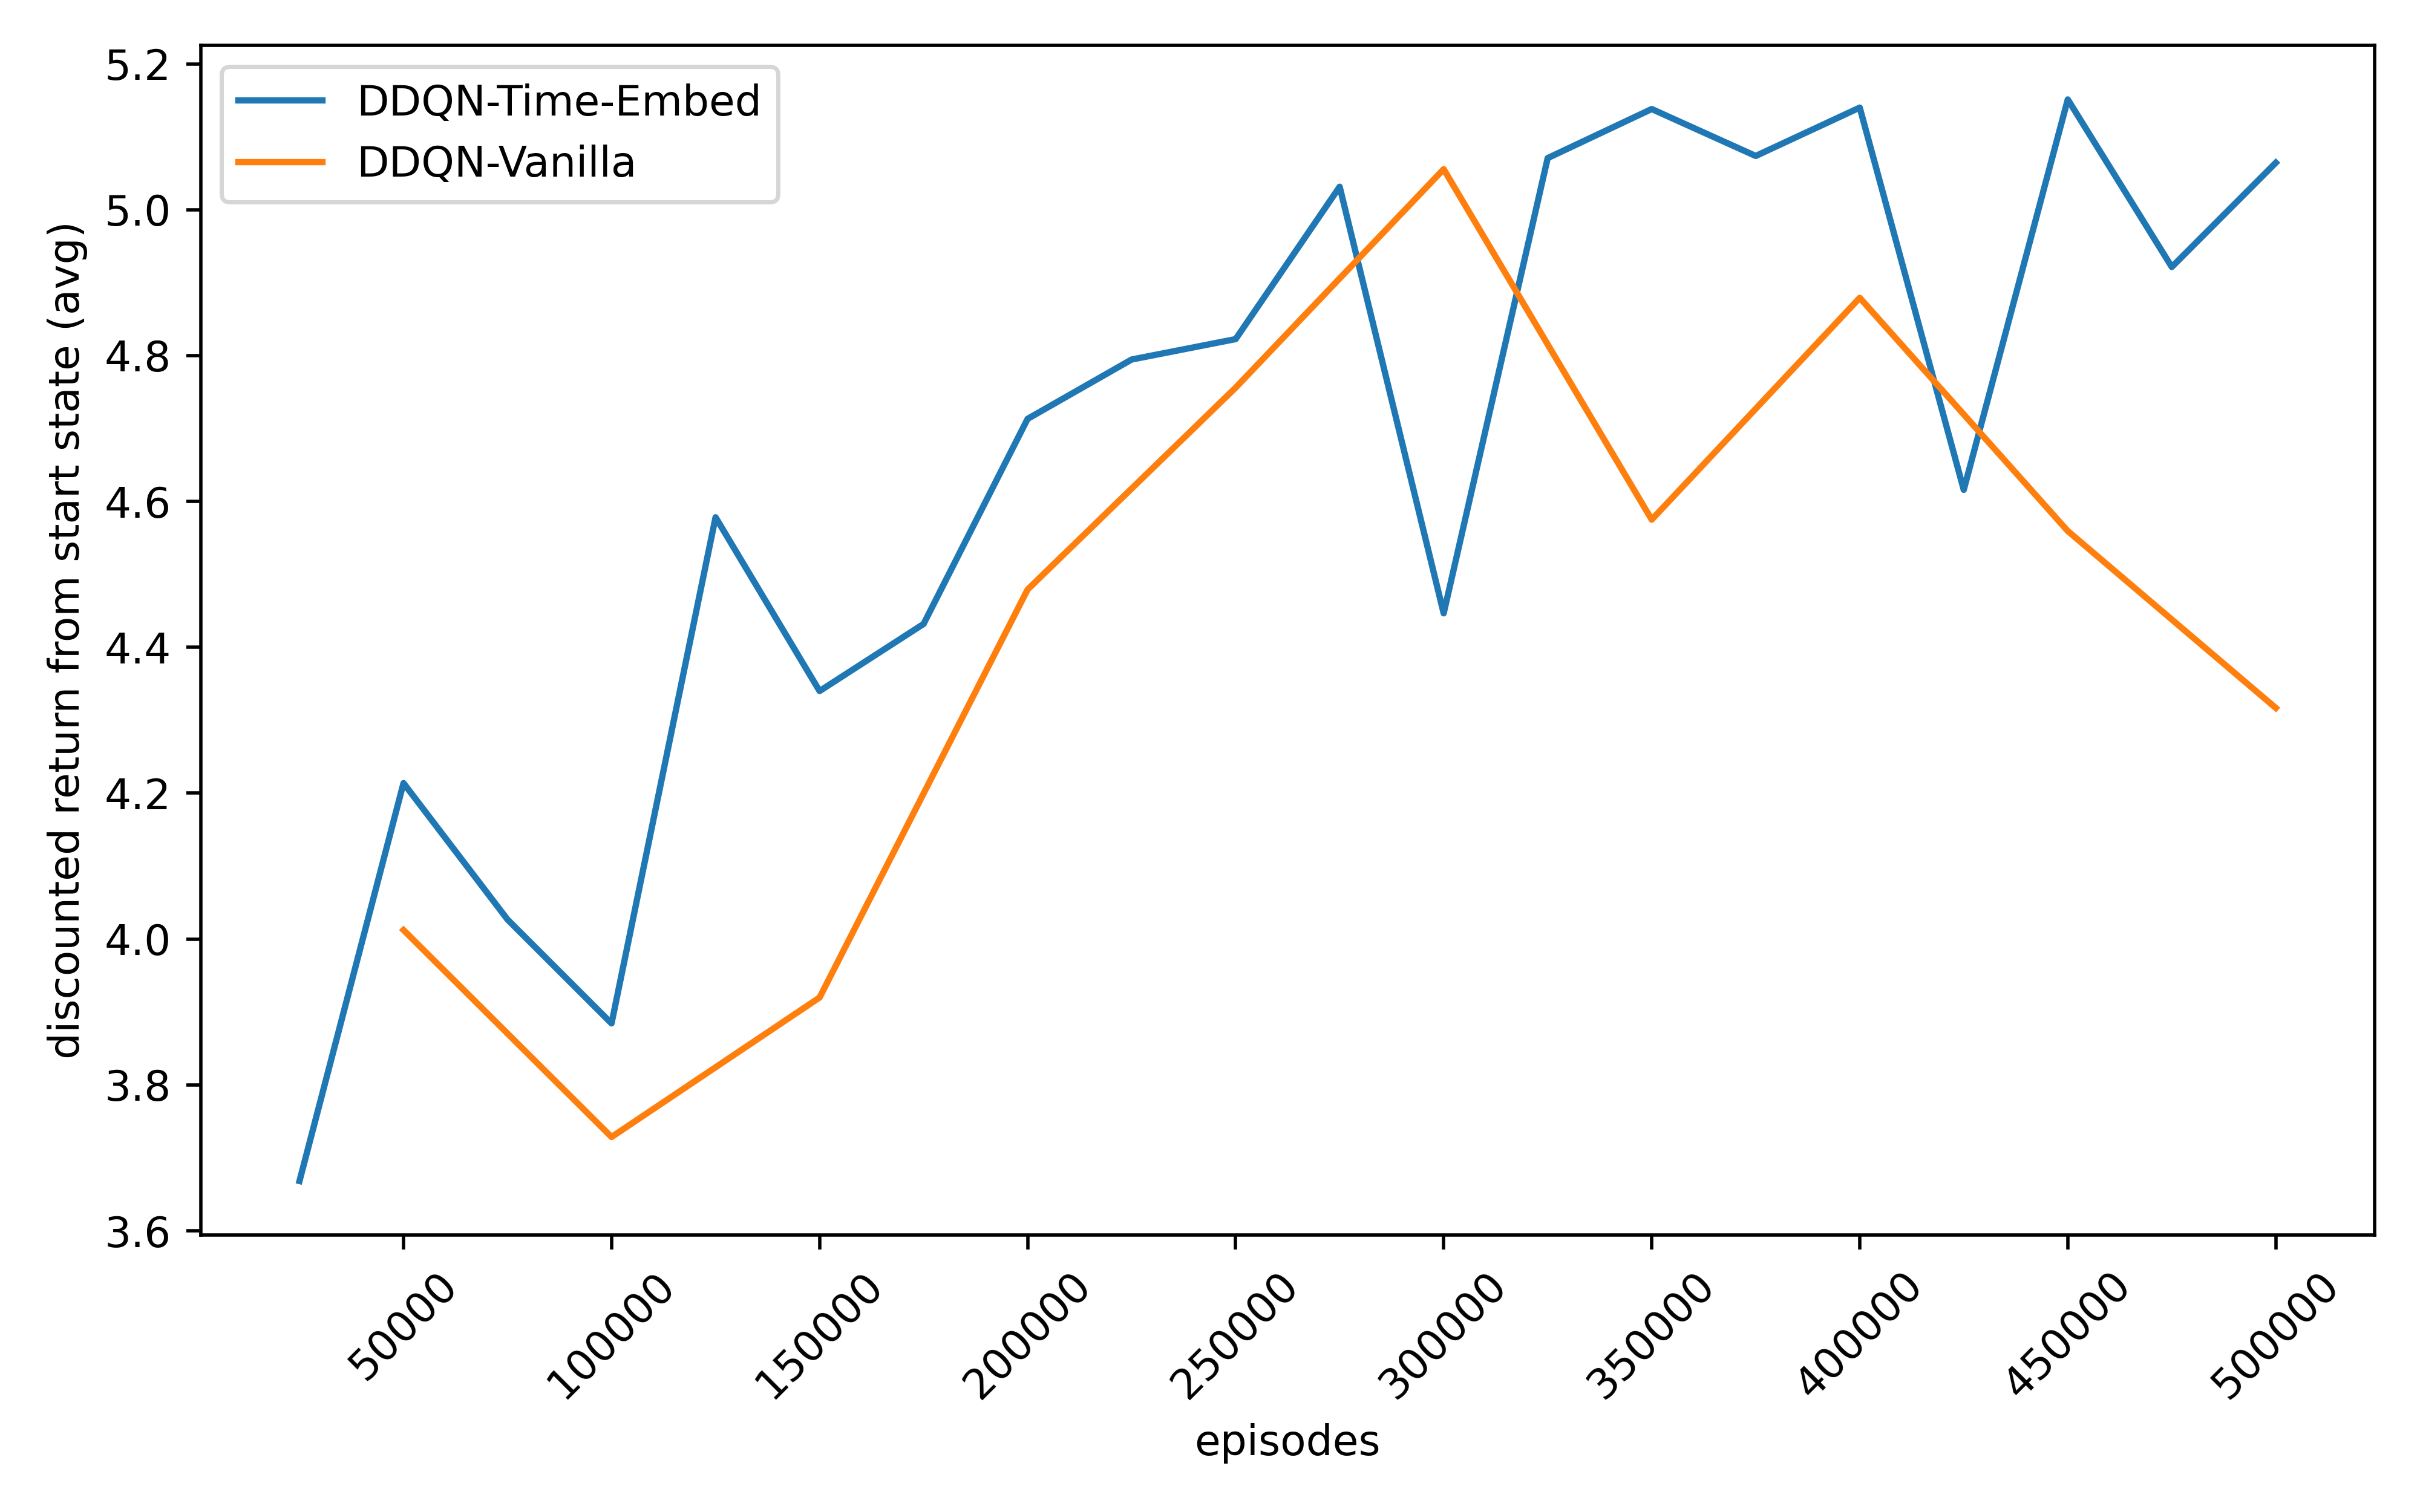
\includegraphics[width=\linewidth]{plots/part3-ddqn-rewards.png}
        \caption{Discounted Return}
    \end{minipage}
    \hfill
    \begin{minipage}{0.32\linewidth}
        \centering
        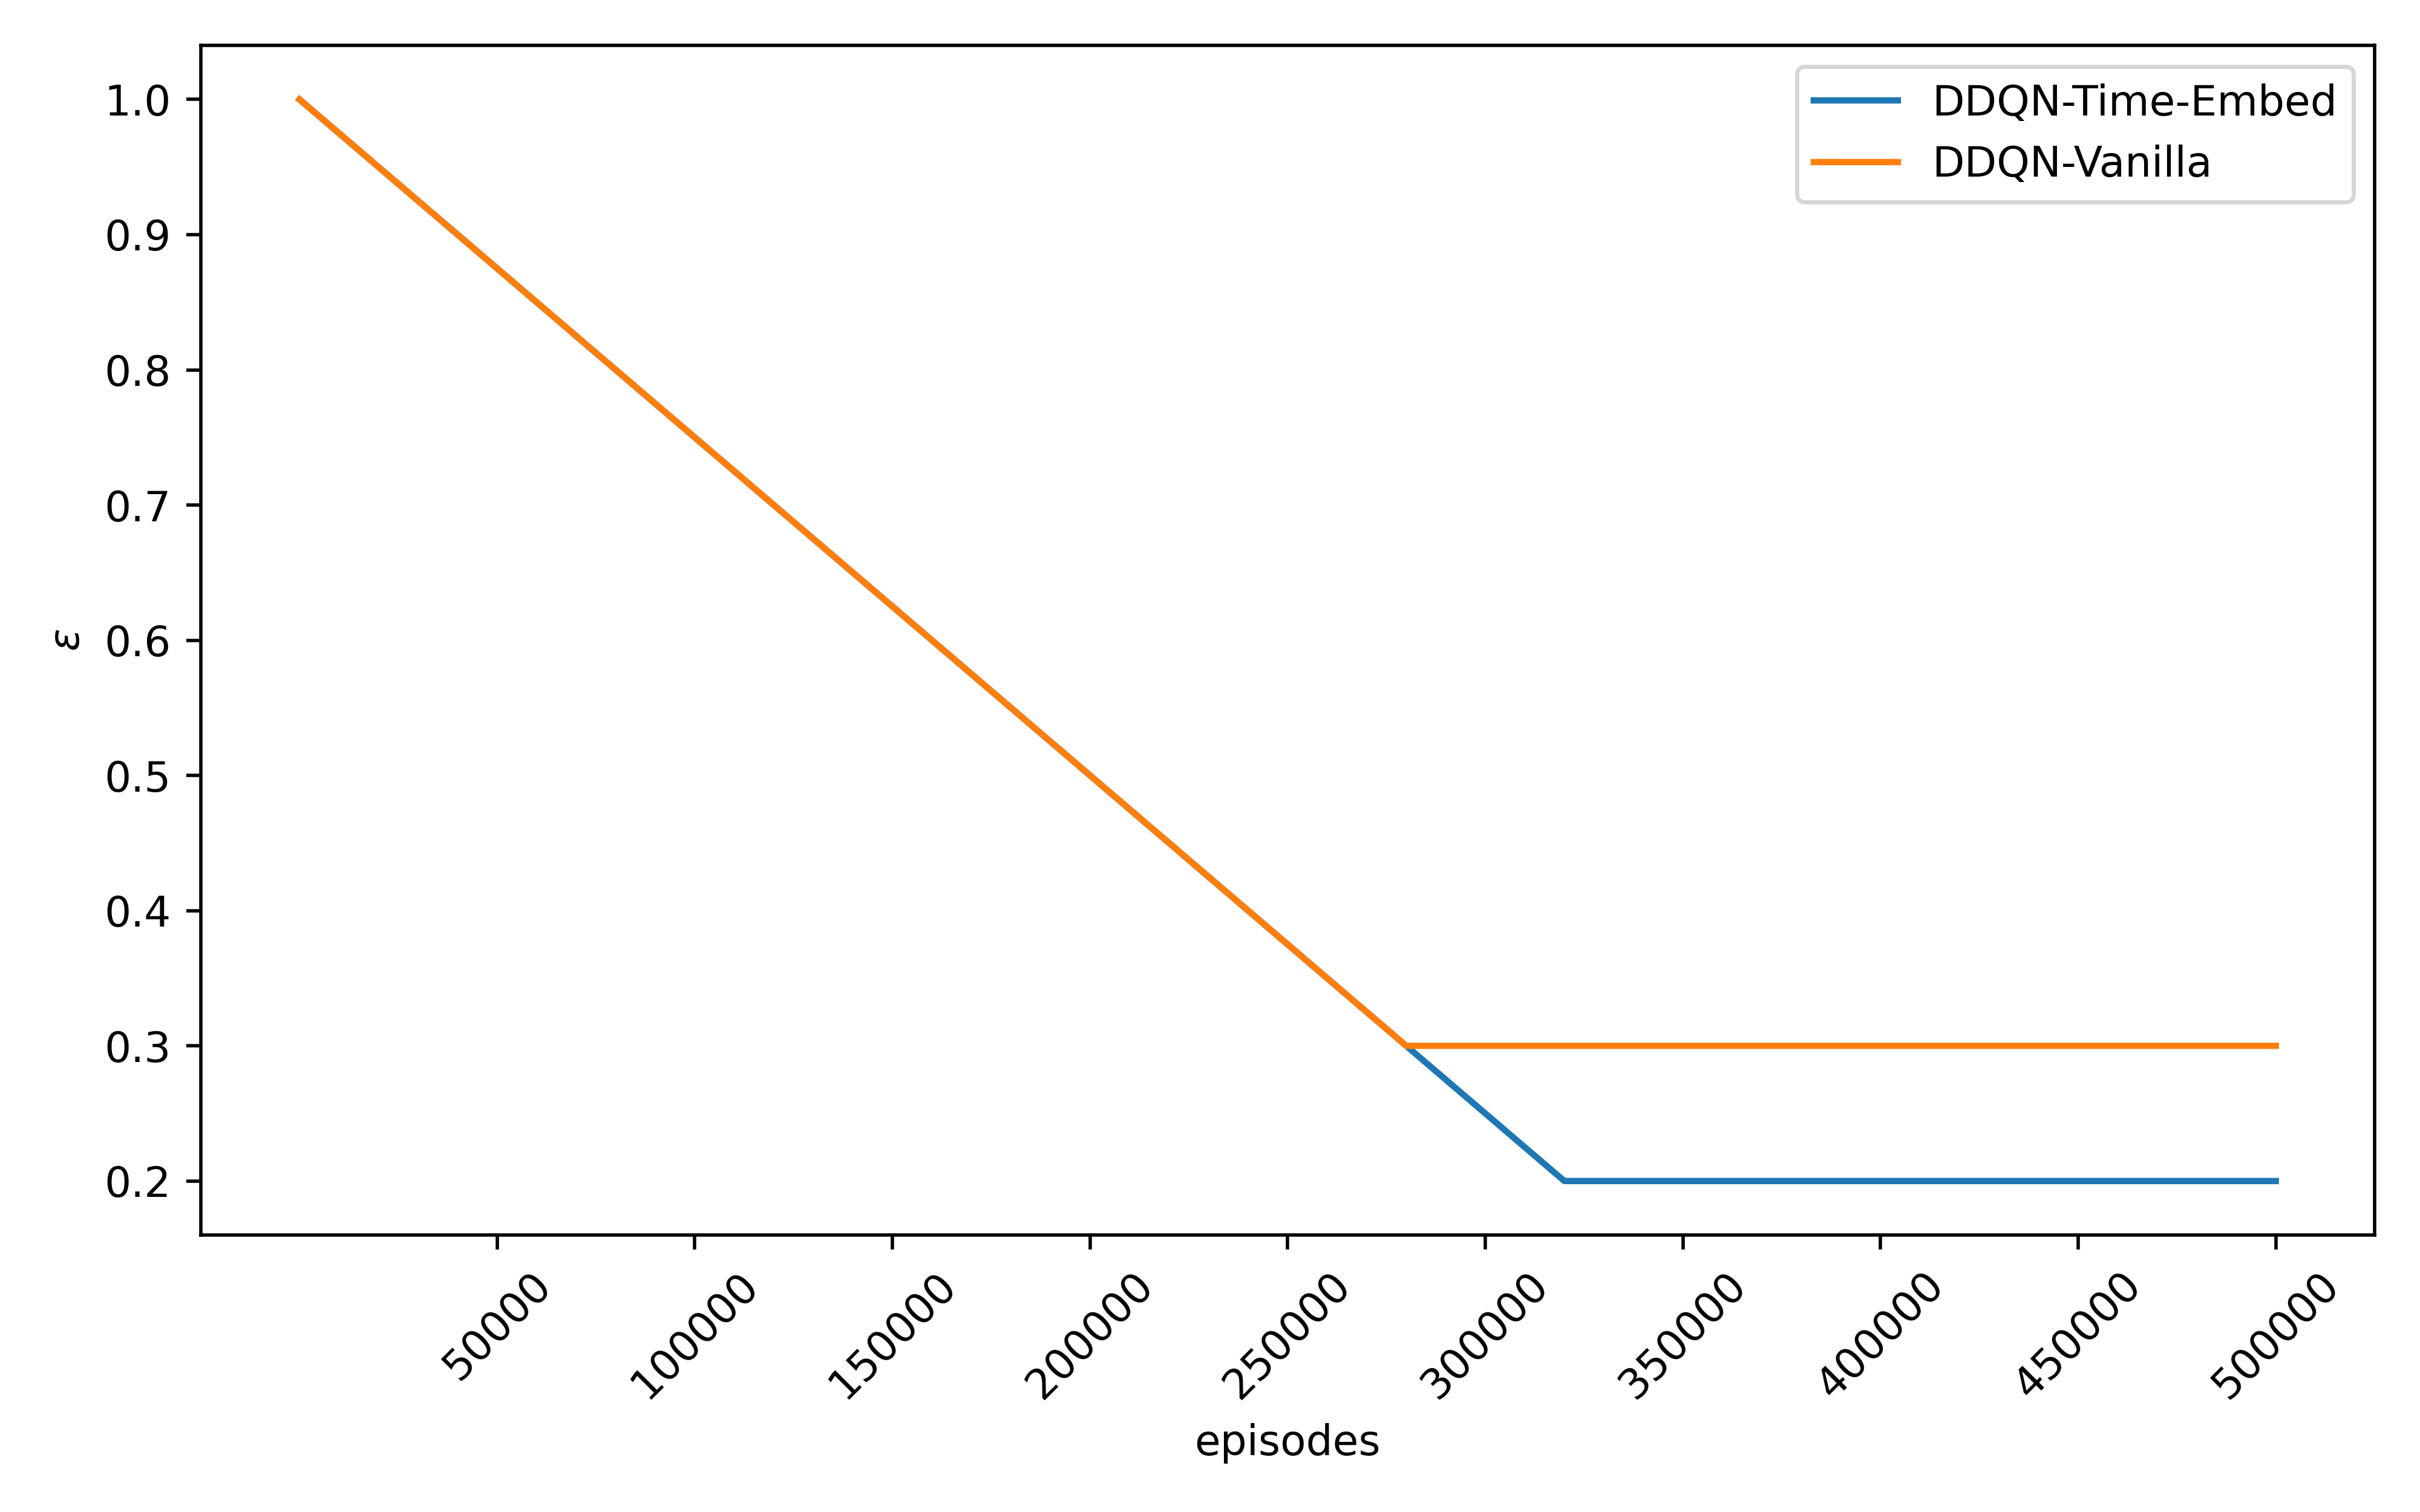
\includegraphics[width=\linewidth]{plots/part3-ddqn-epsilons.png}
        \caption{$\epsilon$ during training}
    \end{minipage}
    \hfill
    \begin{minipage}{0.32\linewidth}
        \centering
        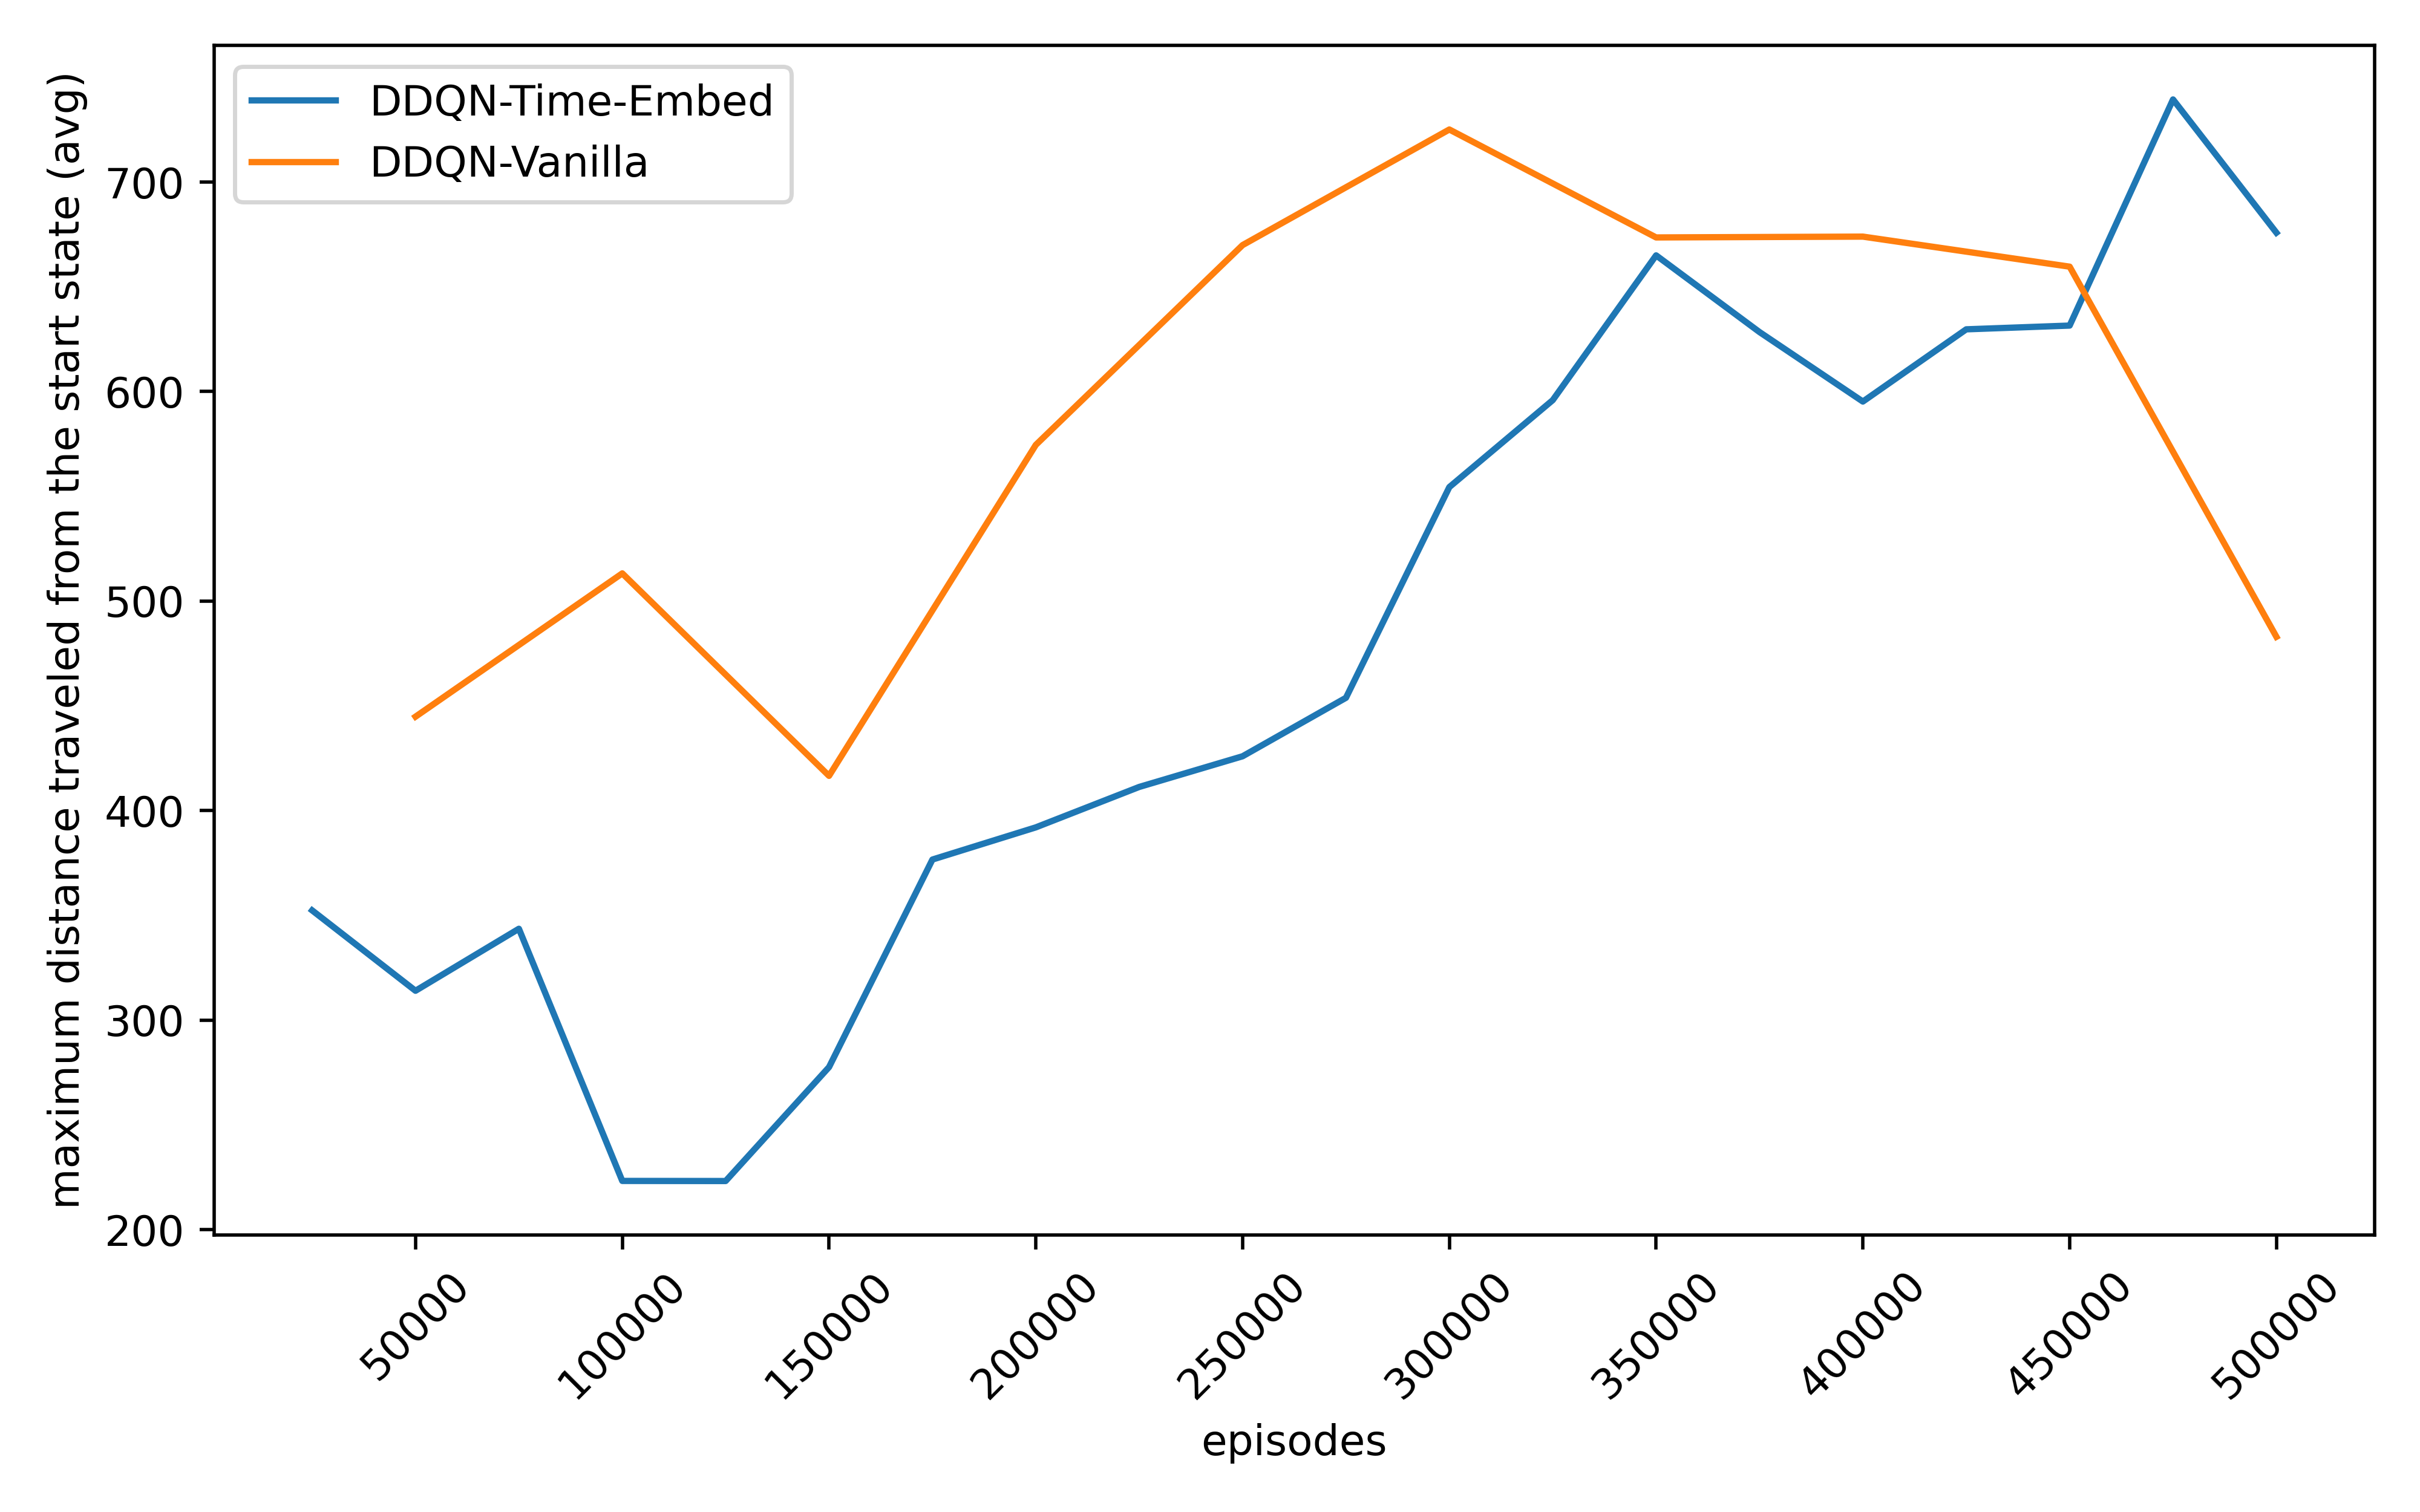
\includegraphics[width=\linewidth]{plots/part3-ddqn-distances.png}
        \caption{Distance Traveled}
    \end{minipage}

    \vspace{0.5em}

    % Second Row - Plots
    \begin{minipage}{0.32\linewidth}
        \centering
        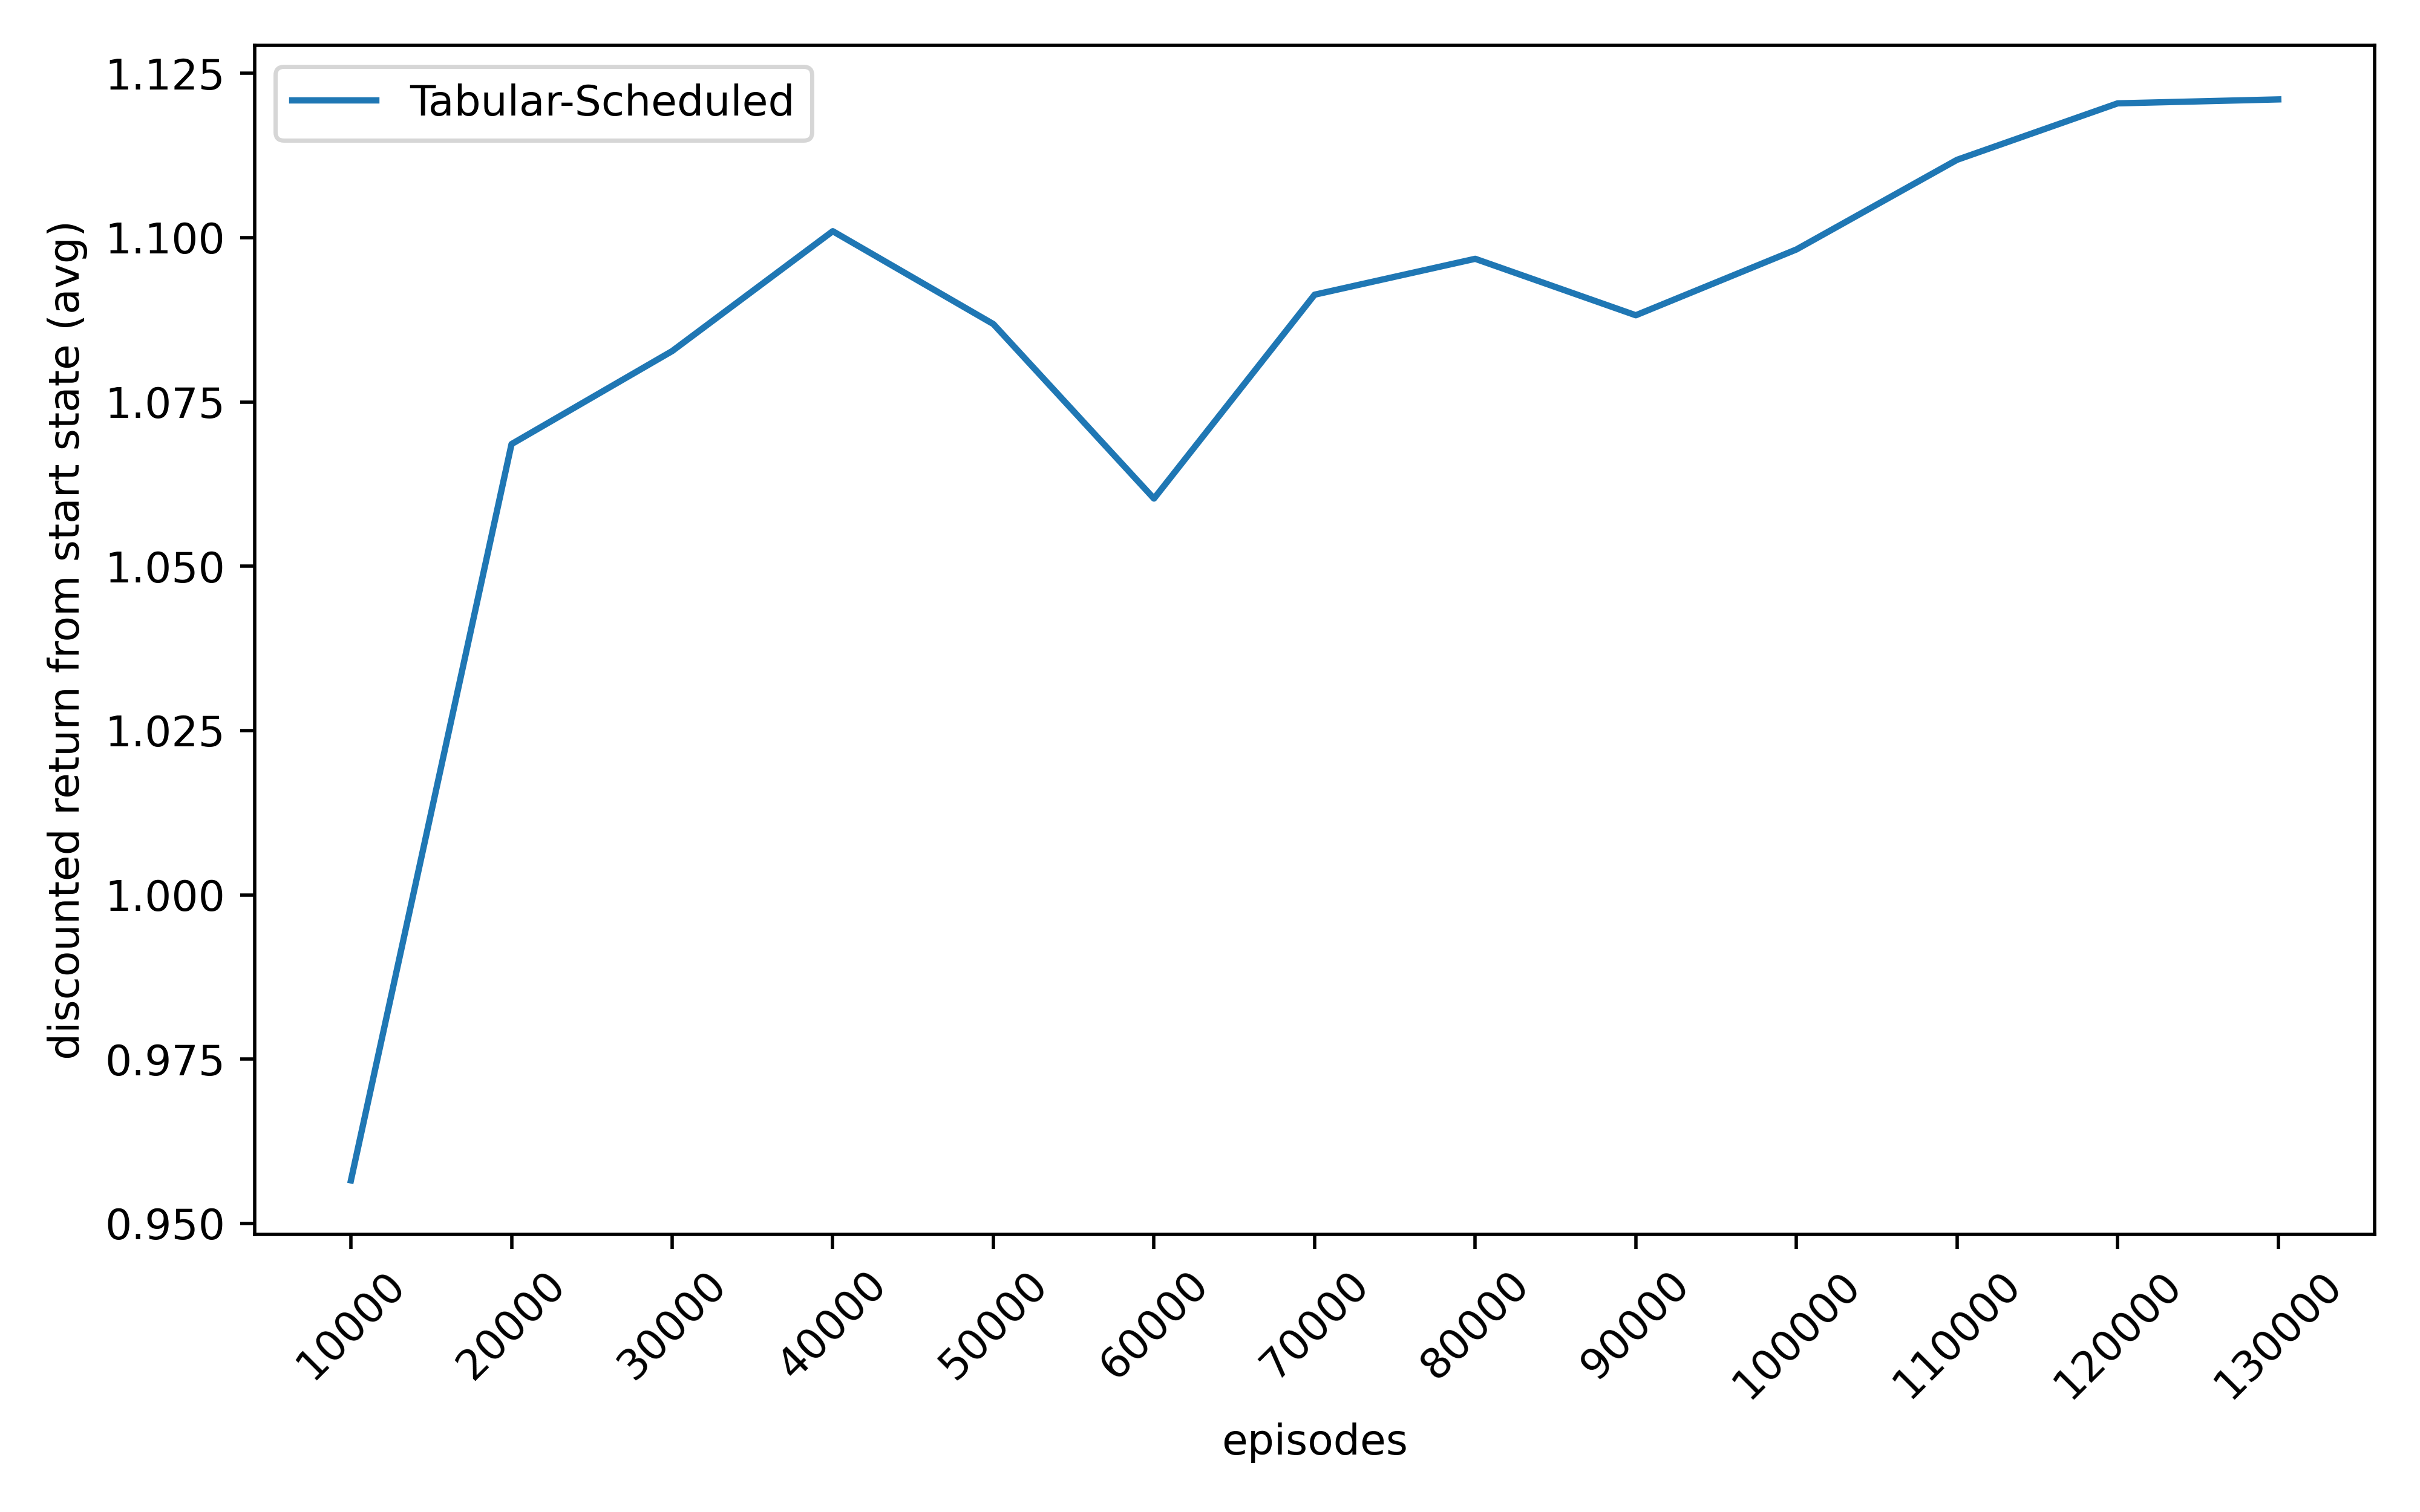
\includegraphics[width=\linewidth]{plots/part3-tabular-rewards.png}
        \caption{Discounted Return}
    \end{minipage}
    \hfill
    \begin{minipage}{0.32\linewidth}
        \centering
        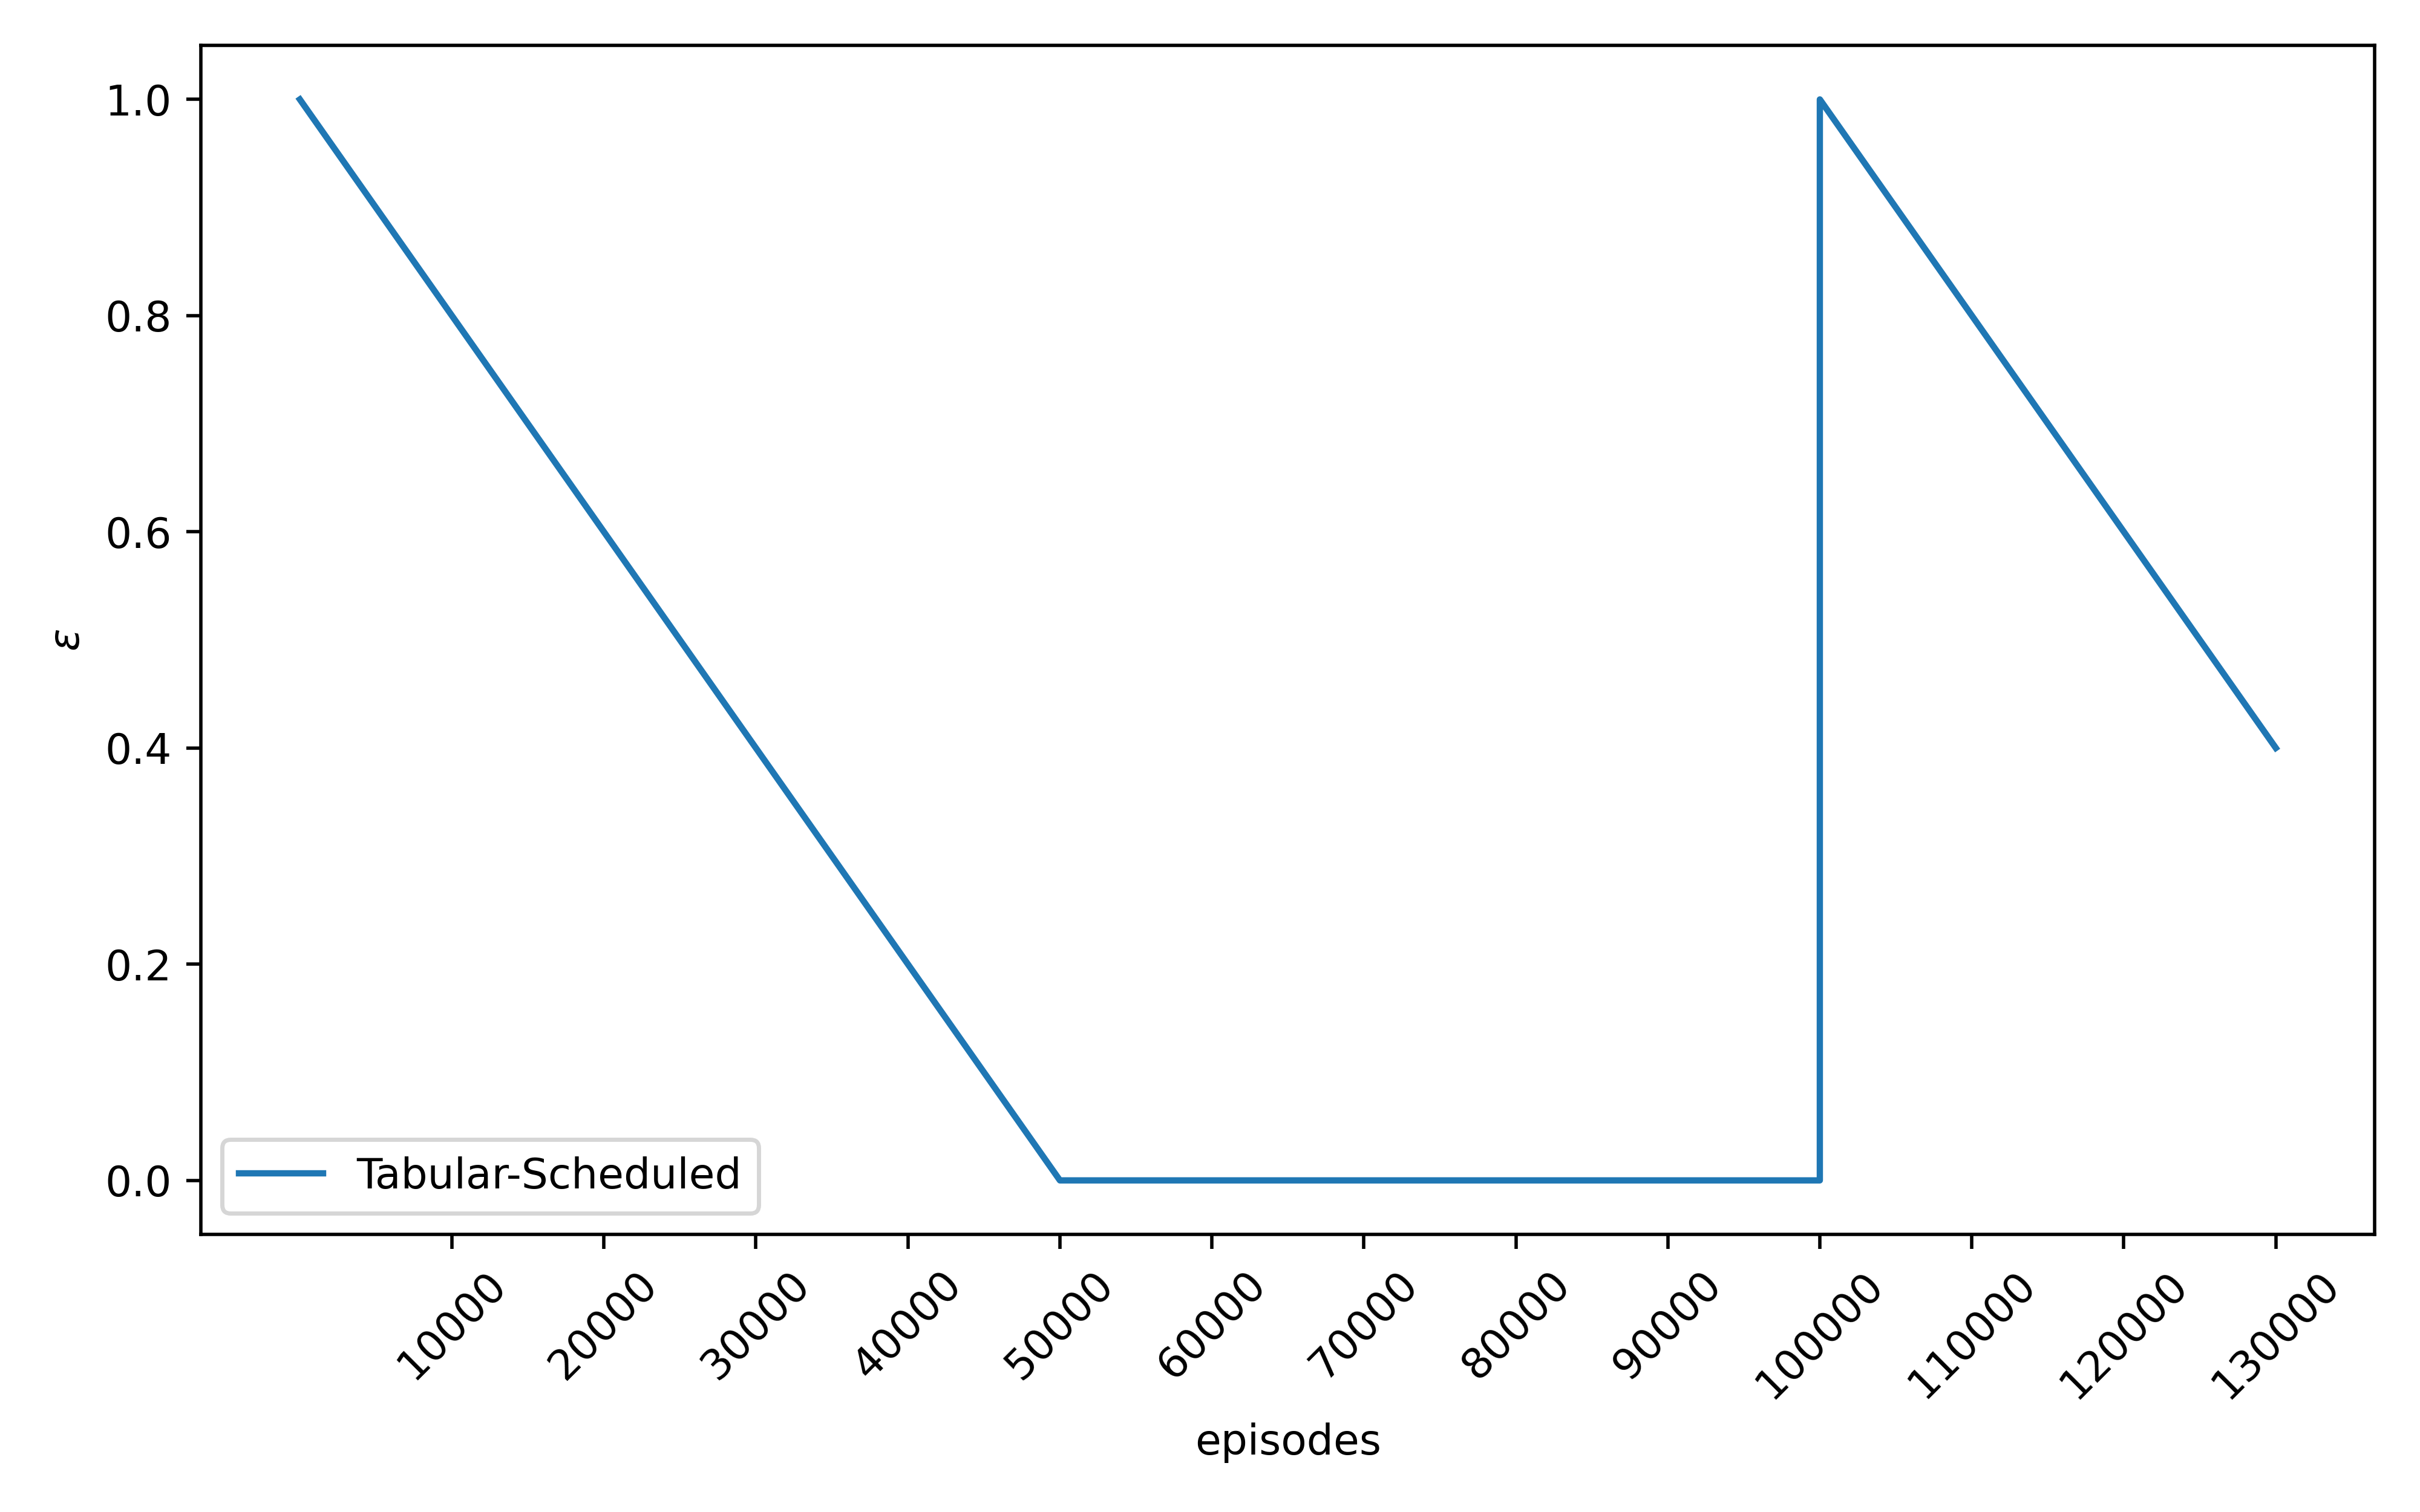
\includegraphics[width=\linewidth]{plots/part3-tabular-epsilons.png}
        \caption{$\epsilon$ during training}

    \end{minipage}
    \hfill
    \begin{minipage}{0.32\linewidth}
        \centering
        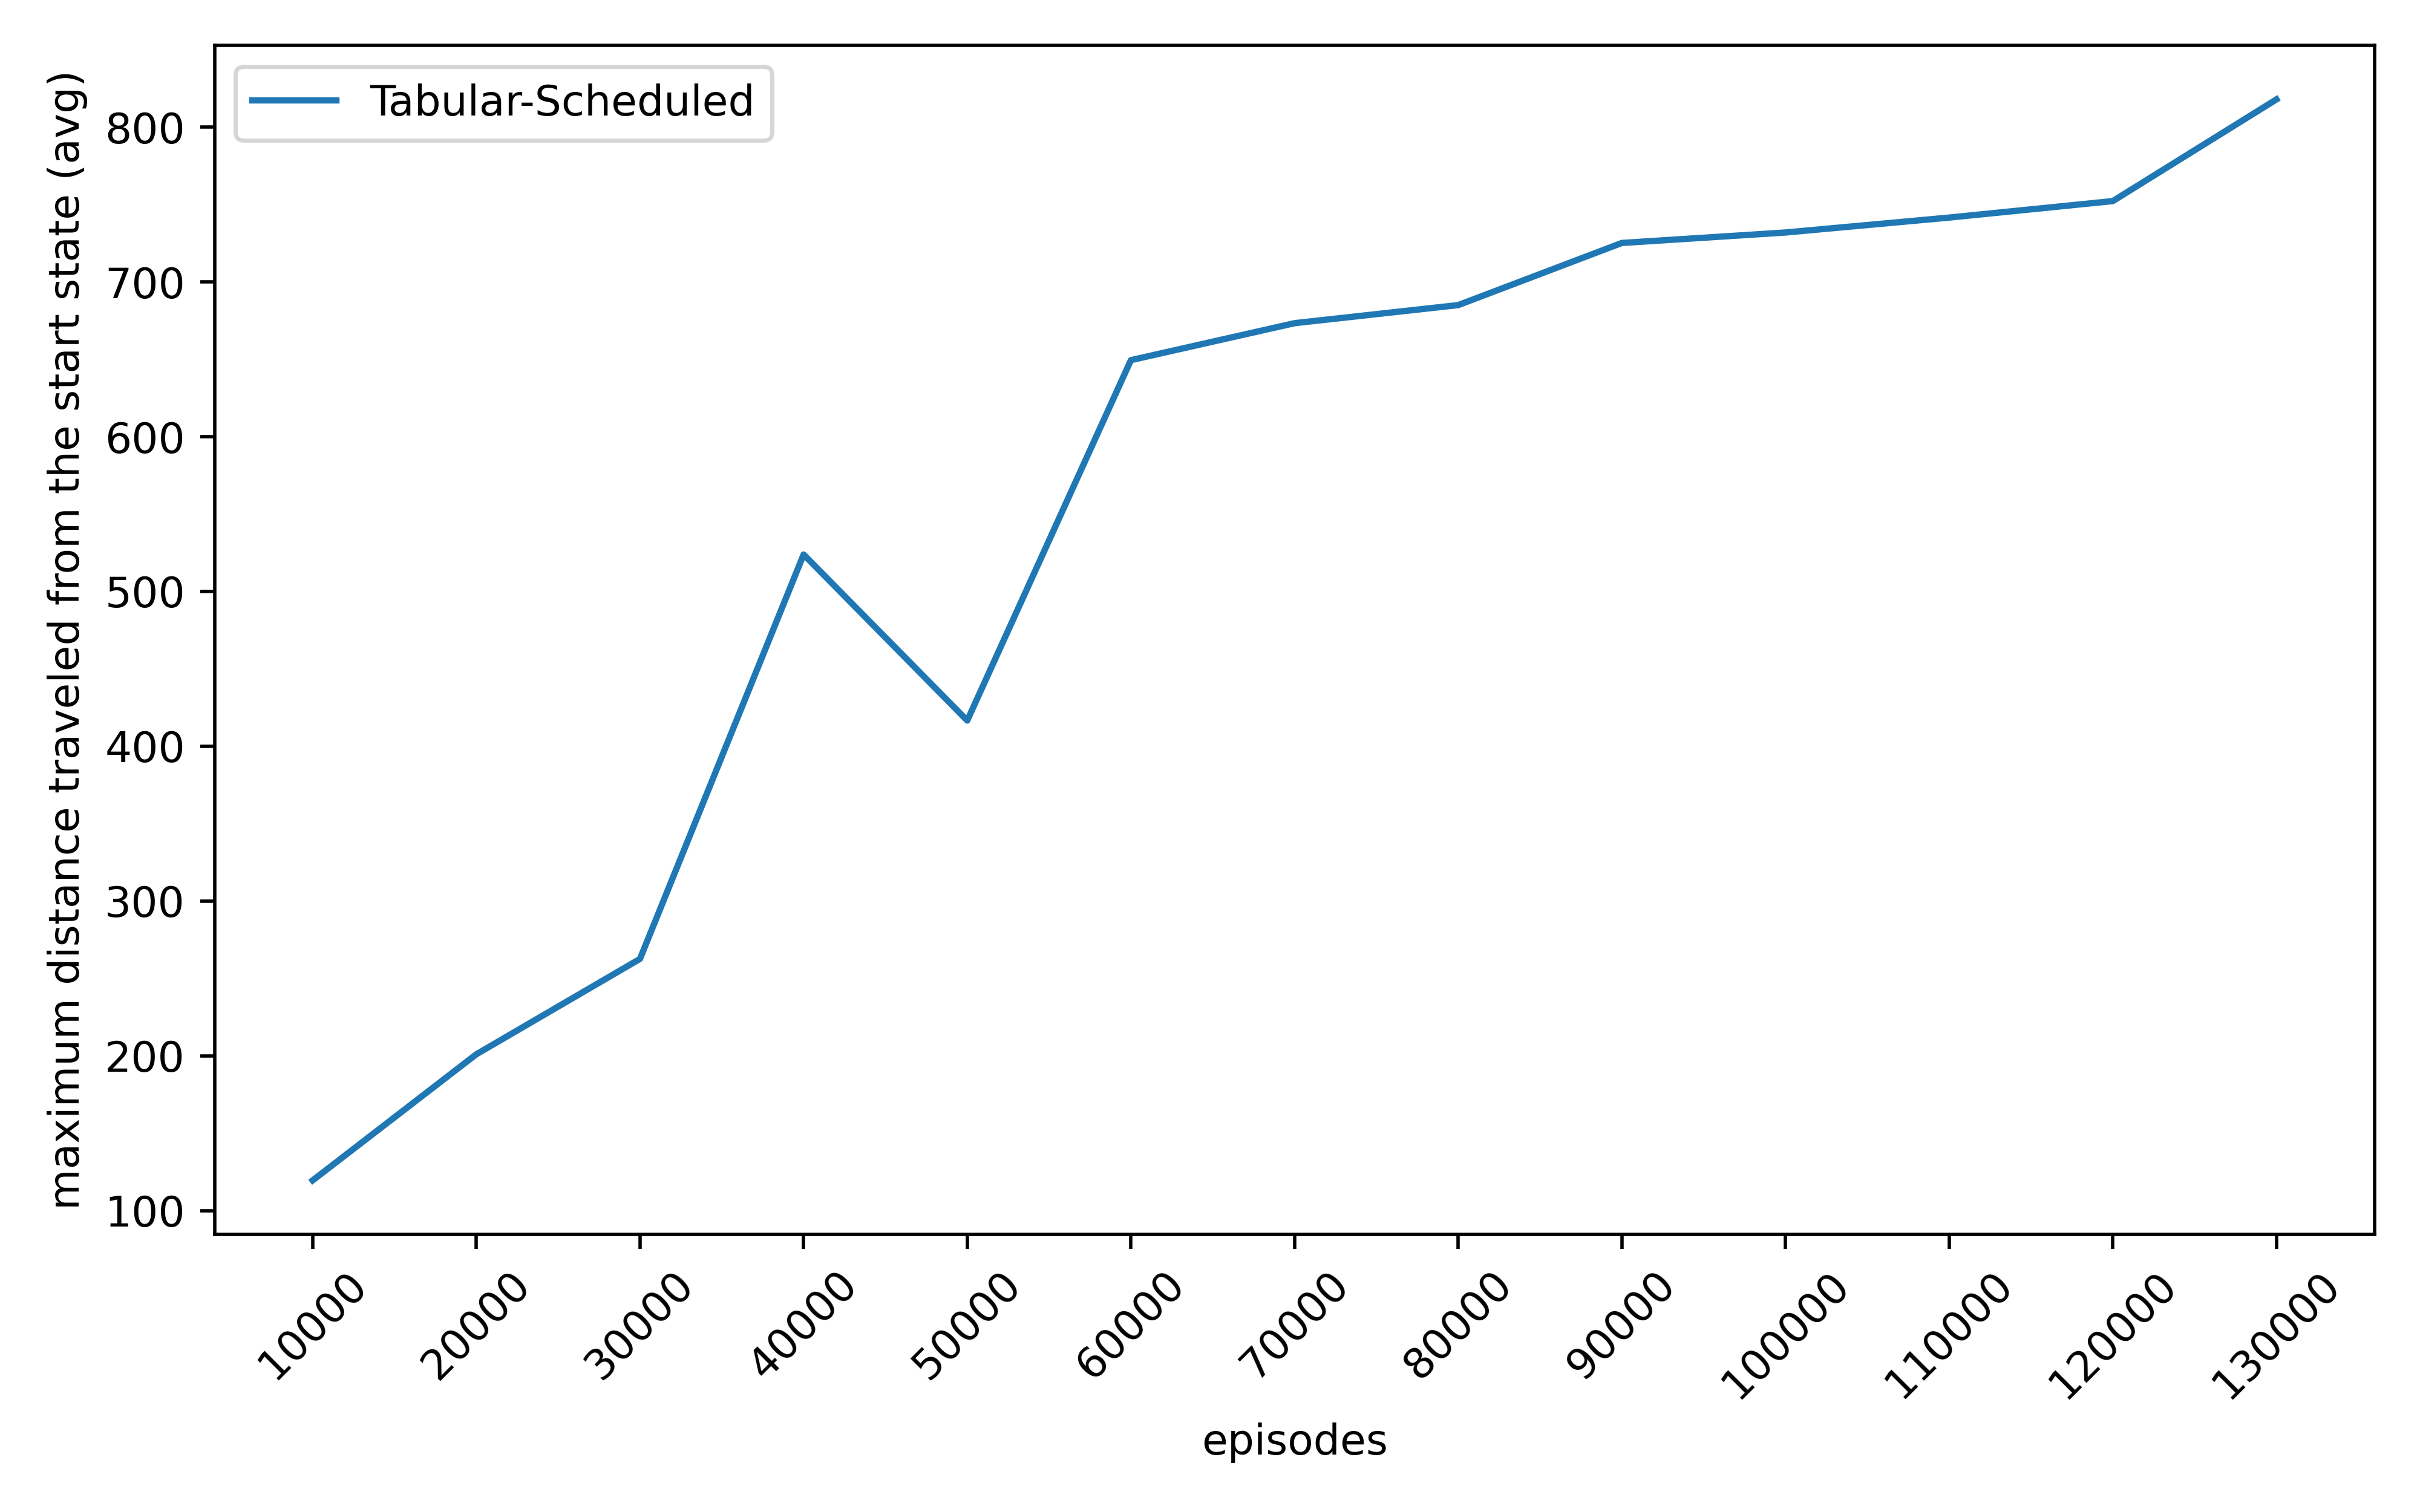
\includegraphics[width=\linewidth]{plots/part3-tabular-distances.png}
        \caption{Distance Traveled}
    \end{minipage}
\end{figure}


\begin{figure}[H]
    \centering

    % Three Tables Side by Side
    \begin{minipage}{0.32\linewidth}
        \centering
        \begin{tabular}{lcc}
            \hline
            Episodes & Discounted & Distance \\
             & Return & Traveled \\
            \hline
            $400,000$ & $5.14$ & $595.23$ \\
            $475,000$ & $4.92$ & $739.43$ \\
            $500,000$ & $5.06$ & $675.82$ \\
            \hline
        \end{tabular}
        \caption{\texttt{DDQN-Time-Embed}}
    \end{minipage}
    \hfill
    \begin{minipage}{0.32\linewidth}
        \centering
        \begin{tabular}{lcc}
            \hline
            Episodes & Discounted & Distance \\
             & Return & Traveled \\
            
            \hline
            $300,000$ & $5.06$ & $725.08$ \\
            $400,000$ & $4.88$ & $673.96$ \\
            $500,000$ & $4.32$ & $482.94$ \\
            \hline
        \end{tabular}
        \caption{\texttt{DDQN-Vanilla}}
    \end{minipage}
    \hfill
    \begin{minipage}{0.32\linewidth}
        \centering
        \begin{tabular}{lcc}
            \hline
            Episodes & Discounted & Distance \\
             & Return & Traveled \\
            \hline
            $50,000$ & $1.09$ & $416.63$ \\
            $100,000$ & $1.10$ & $731.93$ \\
            $130,000$ & $1.12$ & $817.92$ \\
            \hline
        \end{tabular}
        \caption{\texttt{Tabular-Scheduled}}
    \end{minipage}
    \label{fig:part3-time}
\end{figure}

\subsection{Experiments: \texttt{DDQN}}\label{sec:ddqn}
\begin{enumerate}
    \item Both \texttt{DDQN} trained with $\gamma = 0.98, \alpha = 0.1$. \texttt{continuous} observations. The architecture used has the same embedding described in \nameref{sec:arch} but $$64 \texttt{ (input layer)} \to 128 \to 128 \to 64 \to 5 \texttt{ (action layer)}$$ units  respectively in the Neural Network. \texttt{AdamW(lr = 0.0001, amsgrad = True)} is used for training with batch size $512$ and $\tau = 0.005$.

    
    \item \texttt{DDQN-Time-Embed} Reward described in \nameref{sec:reward_design} and $\epsilon$ decreased linearly from $1.0$ to $0.2$ in $320,000$ iterations then kept constant. 
    \item \texttt{DDQN-Vanilla} Reward same as original, \autoref{eqn:reward_vanilla} and $\epsilon$ decreased linearly from $1.0$ to $0.3$ in $280,000$ iterations then kept constant.

    \item Neither of these models would fit in the $2$-hours time limit, and the training time also make it difficult to discover hyper-parameters.
\end{enumerate}
\subsection{\texttt{BestAgent: Tabular-Scheduled}}
\begin{enumerate}
\item We trained the \texttt{Tabular} agent for $100,000$ episodes with $\gamma =  0.90, \alpha = 0.1$ and $\epsilon$ decreased linearly from $1.0$ to $0.0$ in $50,000$ episodes. After $100,000$ episodes we train it with $\gamma = 0.90, \alpha = 0.01$ for $30,000$ episodes. $\epsilon$ follows the same schedule as before.
\item Over $100,000$ seeds from $0$ to $99,999$, the \texttt{Tabular-Scheduled} policy gave an average distance $812.11$ with standard deviation $276.30$. 
\end{enumerate}